\section{Conclusion}
From the turbulence energy, pressure and $z-$velocity, it can be concluded that it is not around the Flatiron building but around the building behind the Flatiron skyscraper that the women's skirts have a chance to billow. The wind speed in the $z-$direction is a little higher than 1.1 ms$^{-1}$, which would not make the women's skirts fly up. However, at that corner there is a high concentration of turbulence kinetic energy, making it possible that the wind speed increases and catch the women's skirts. This updraft and kinetic energy is partly caused by the air splitting at the tip of triangular geometry of the Flatiron building, and coming together on the other side, as well as the geometry and placement of the surrounding buildings.

\section{Recommendations}
\begin{itemize}
\item To simplify the geometry, the building behind the Flatiron building was taken to be rectangular. However, it is clear that this building plays a large role in the turbulent area behind the Flatiron building. To higher the accuracy of the CFD analysis, we recommend to use a finer discretization, or make a true straight wall (so implement an obstacle creator with tilted obstacles).

\item Since we were limited in the hardware to use for the simulations, we were also limited in the complexity of the environment and mesh. Using a machine with more than 2 GB of RAM allows for more detailed results to be post-processed. 

\item The air is already deflecting at the first plane after entering, which shows that it might be better to take a bigger area in front of the building. 

\item The visualization tools only had a resolution of 1.37~m in the $z-$direction, even though the mesh had a size of 0.1~m on the floor. It would be nice to visualize the air below 1.37~m as well, since this is the area of interest for women's skirts. 

\item We recommend men visiting the Flatiron building to stand across the street, as indicated by the red dot in \autoref{fig:recommendation}. This will give a nice view of the most probable place of any action happening. 
\end{itemize}

\begin{figure}[htbp]
	\centering
		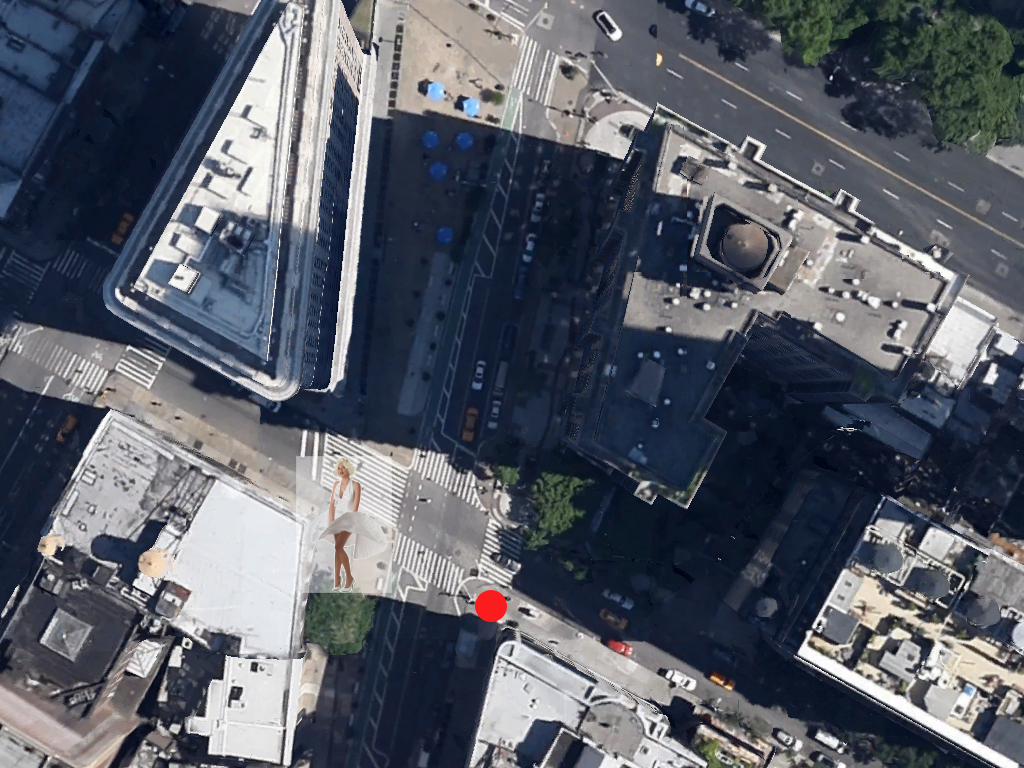
\includegraphics[width=0.80\textwidth]{recommendation.png}
	\caption{The red dot indicates a place with a good view on billowing skirts.}
	\label{fig:recommendation}
\end{figure}
